\documentclass[tikz, border=10pt]{standalone}
% cf http://cloford.com/resources/colours/websafe1.htm
\definecolor{sv-all}{RGB}{255,153,255}
\definecolor{sv-gxe-m2}{RGB}{255,204,255}
\definecolor{sv}{RGB}{255,153,255}
\definecolor{m1}{RGB}{153,153,255}
\definecolor{m2}{RGB}{153,255,153}
\definecolor{ge}{RGB}{255,255,153}
\definecolor{sp}{RGB}{255,153,153}
\definecolor{vi}{RGB}{255,204,153}
\definecolor{ma}{RGB}{204,255,153}
\definecolor{hedo}{RGB}{153,153,255}
\definecolor{nap}{RGB}{153,255,153}

\usetikzlibrary{
  mindmap,
  decorations.pathreplacing,    % paths with shoapes of curly braces
  positioning,     % positions like above of node
  fit              % legend bounding box fitting all nodes
}
\tikzset{
  node distance=4ex and 4ex,
  % on grid,  % node distance from the centers
  every node/.style = {
    rectangle,
    minimum width=5em,
    minimum height=3ex,
    text depth=1pt,
    draw,
    outer sep = 2pt,
    inner sep = 3pt
  },
  every edge/.style = {->,draw},
  virtual/.append style = {draw=none, circle, minimum width=1em},
  % virtual/.append style = {draw, color=black!50},   % debugging purposes
  several-all/.append style = {fill = sv-all},
  several-gxe-m2/.append style = {fill = sv-gxe-m2},
  m1/.append style = {fill = m1},
  m2/.append style = {fill = m2},
  gxe/.append style = {fill = ge},
  sp/.append style = {fill = sp},
  vi/.append style = {fill = vi},
  ma/.append style = {fill = ma},
  aux/.append style = {fill = none},
  hedo/.append style = {fill = hedo},
  nap/.append style = {fill = nap},
  legendkey/.append style = {minimum width=3ex},
  legendtext/.append style = {draw=none, fill = black!10},
  ->,        % arrows for all
  >=stealth  % arrow type
}
\pgfdeclarelayer{background}
\pgfsetlayers{background,main}


\begin{document}

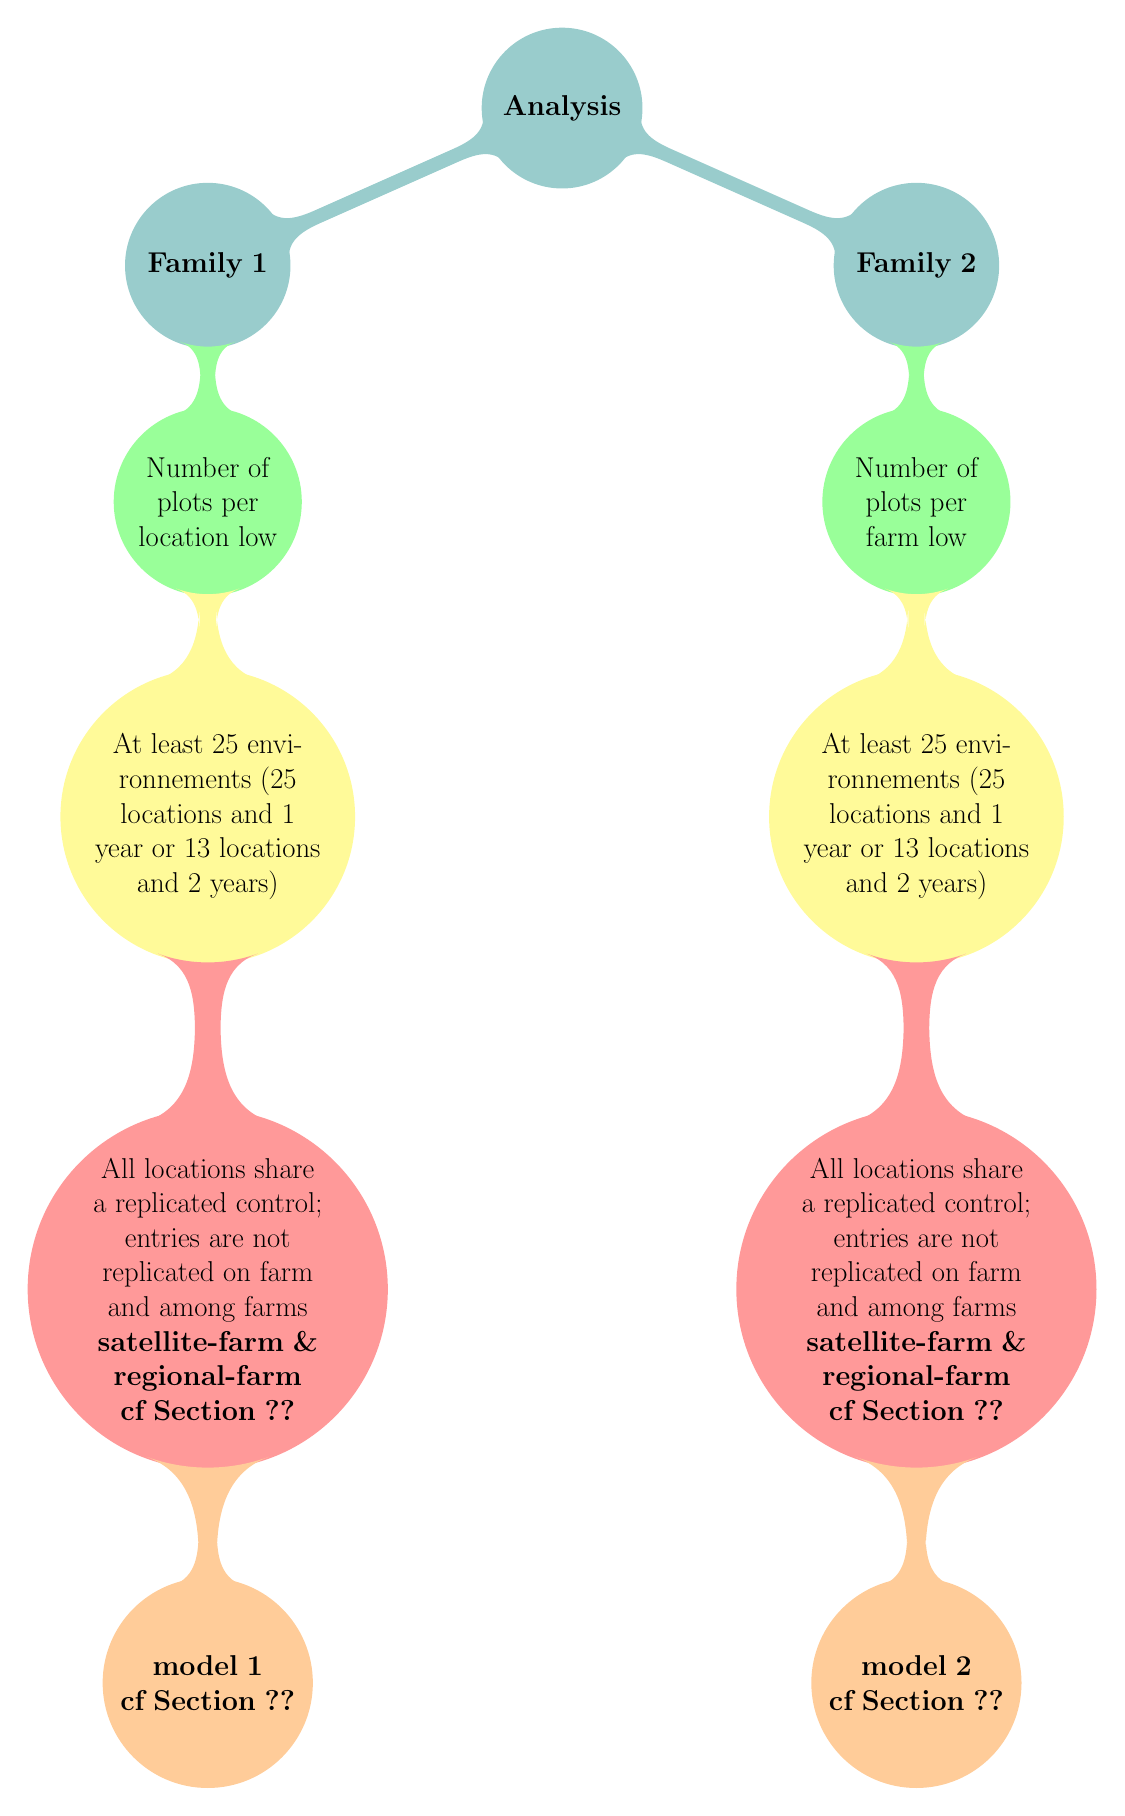
\begin{tikzpicture}[mindmap,
every node/.style=concept, concept color=teal!40,
every node/.append style={scale=0.5},
%every concept/.style={rectangle},
    level 1/.style={level distance=2cm, sibling distance= 9cm, concept color=teal!40, font=\huge, text width=4cm},
    level 2/.style={level distance=3cm, sibling distance= 9cm, concept color=green!40, font=\huge, text width=4cm},
    level 3/.style={level distance=4cm, sibling distance= 4cm, concept color=yellow!40, font=\huge, text width=6cm},
    level 4/.style={level distance=6cm, concept color=red!40, font=\huge, text width=6cm},
    level 5/.style={level distance=5cm, sibling distance= 3cm, concept color=orange!40, font=\huge, text width=5cm},
    ]

\node{ \huge \textbf{Analysis} }
      child { node {\textbf{Family 1}}
        child { node {Number of plots per location low}
       		child { node {At least 25 environnements (25 locations and 1 year or 13 locations and 2 years)}
        		child { node { All locations share a replicated control; entries are not replicated on farm and among farms \\ \textbf{satellite-farm \& regional-farm \\ cf Section~\ref{rf_sf}} }
	      			child { node {\textbf{model 1 \\ cf Section~\ref{model_1}}} }
        		}
       		}
		    }
      }
      child { node {\textbf{Family 2}}
        child { node {Number of plots per farm low}
        	child { node {At least 25 environnements (25 locations and 1 year or 13 locations and 2 years)}
        		child { node { All locations share a replicated control; entries are not replicated on farm and among farms \\ \textbf{satellite-farm \& regional-farm \\ cf Section~\ref{rf_sf}} }
					child { node {\textbf{model 2 \\ cf Section~\ref{model_2}} }}
	        	}
        	}
        }
      };
\end{tikzpicture}

\end{document}
